\title{Lausn á \emph{Pipe Rotation}}
\author{Bergur Snorrason}
\date{\today}

\begin{document}

\frame{\titlepage}

\env{frame}
{
	\env{itemize}
	{
		\item<1-> Okkur er gefið $n \times m$ ($1 \leq n, m \leq 100$) borð af spilum af eftirfarandi gerðum:
		\item<2->[] 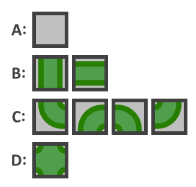
\includegraphics[scale = 0.25]{fig/pr1}
		\item<3-> Við eigum að ákvarða hvort hægt sé að snúa spilunum þannig að allar hliðar sem eru grænar eru gagnstæðar hliðum sem eru einnig grænar.
		\item<4-> Takið eftir að við megum ekki endurraða spilunum og að hliðar sem snúa út mega ekki vera grænar.
	}
}

\env{frame}
{
	\env{itemize}
	{
		\item<1-> Sjáum dæmi.
		\item<2->[] 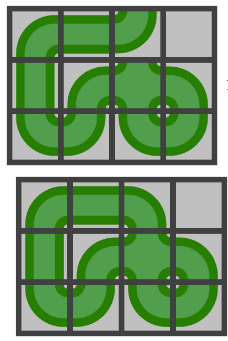
\includegraphics[scale = 0.25]{fig/pr2}
		\item<3-> Efra dæmið er ekki löglegt en neðra er löglegt.
	}
}

\env{frame}
{
	\env{columns}
	{
		\env{column}
		{
			{0.8\textwidth}
			\env{itemize}
			{
				\item<1-> Sjáum fyrst að ef við vitum hvað er vinstra megin og fyrir ofan spil þá vitum við hvernig það þarf að snúa.
				\item<2-> Ef hliðin fyrir ofan er auð og hliðin til vinstri er auð þá þarf spilið að vera af gerð \texttt{A}
							eða af gerð \texttt{C} í öðrum snúning.
				\item<3-> Ef hliðin fyrir ofan er auð og hliðin til vinstri er græn þá þarf spilið að vera af gerð \texttt{B} í seinni snúning
							eða af gerð \texttt{C} í þriðja snúning.
				\item<4-> Ef hliðin fyrir ofan er græn og hliðin til vinstri er auð þá þarf spilið að vera af gerð \texttt{B} í fyrri snúning
							eða af gerð \texttt{C} í fyrsta snúning.
				\item<5-> Ef hliðin fyrir ofan er græn og hliðin til vinstri er græn þá þarf spilið að vera af gerð \texttt{C} í fjórða snúning
							eða af gerð \texttt{D}.
			}
		}
		\env{column}
		{
			{0.2\textwidth}
			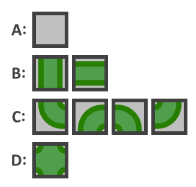
\includegraphics[scale = 0.3]{fig/pr1}
		}
	}
}

\env{frame}
{
	\env{itemize}
	{
		\item<1-> Nú getum við labbað í gegnum öll spilin og ákvarðað hvernig hvert spil snýr ef við byrjum á efstu línunni og vinnum okkur niður,
					og skoðum hverja línu frá vinstri til hægri.
		\item<2-> Það er pínu vinna að útfæra þetta útaf öllum tilfellunum sem þarf að hafa í huga.
	}
}

\env{frame}
{
	\selectcode{code/piperotation.c}{4}{8}
}

\env{frame}
{
	\selectcode{code/piperotation.c}{10}{47}
}

\env{frame}
{
	\env{itemize}
	{
		\item<1-> Þessi lausn er lítið annað en tvöföld \texttt{for}-lykkja sú ytri af lengd $n$ og sú innri af lengd $m$.
		\item<2-> Svo tímaflækjan er $\mathcal{O}($\onslide<3->{$n \cdot m$}$)$.
	}
}

\env{frame}
{
}

\end{document}
